\begin{frame}
    \frametitle{Why Generation IV Reactors?}
    \begin{itemize}
      \item Energy use and production contribute $\frac{2}{3}$ of Greenhouse Gas 
      emissions \cite{noauthor_climate_2018}
      \item  Large scale emissions-free nuclear power deployment could 
      significantly reduce GHG production but faces both cost and perceived 
      safety challenges 
      \item The Generation IV International Forum identified six systems 
      that promise significant advances in safety, sustainability, efficiency, 
      and cost over existing designs: GFR, LFR, MSR, SFR, SCWR, and VHTR. 
      \begin{figure}[htbp!]
          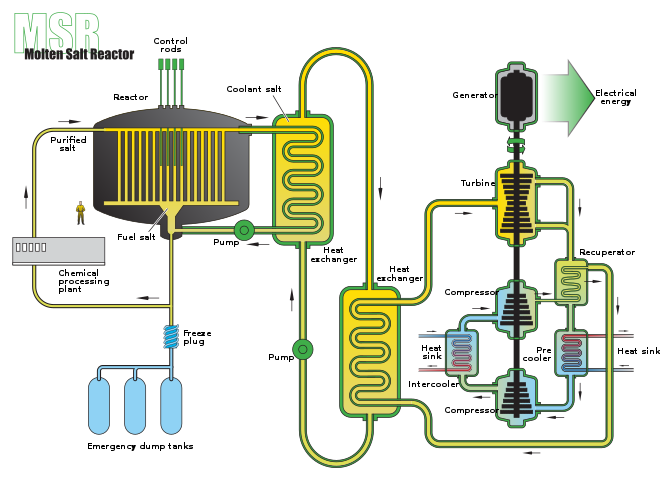
\includegraphics[height=3cm]{figures/msr}
          \hspace{1cm}
          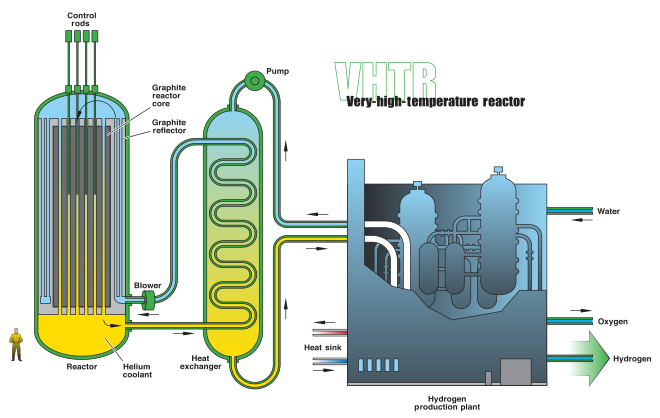
\includegraphics[height=3cm]{figures/vhtr}
          \caption{Left: Molten Salt Reactor System, Right: Very High-Temperature
          Reactor System \cite{gif_technology_2002}. }
      \end{figure}
    \end{itemize}
  \end{frame}
\begin{frame}
  \frametitle{MSRs and VHTRs}
  \begin{block}{Molten Salt Reactor (MSR) System Advantages}
    \begin{itemize}
      \item Molten Fluoride Salts: chemical stability, low vapor pressure at 
      high temperatures, good heat transfer, resistance against radiation damage
      \item Inherent System Safety: passive cooling, fail-safe drainage
    \end{itemize}
  \end{block}
  \vspace{-0.25cm}
  \begin{block}{Very High Temperature Reactor (VHTR) System Advantages}
    \begin{itemize}
      \item TRISO Fuel: withstands high burnup and temperature
      \item High Outlet Temperature: increases power conversion efficiency, reduces 
      waste heat generation, enables high-temperature heat applications 
    \end{itemize}
  \end{block}
  \begin{figure}[htbp!]
    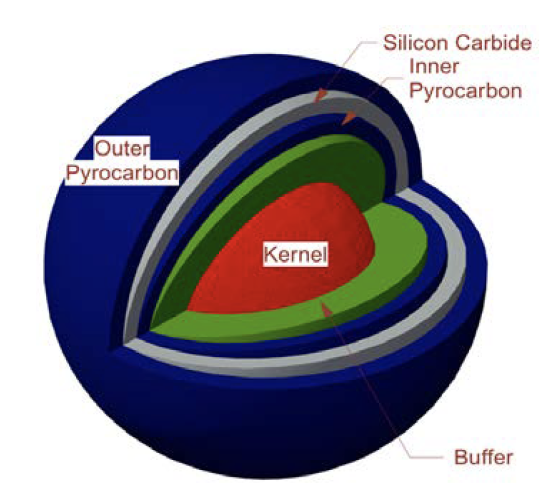
\includegraphics[width=0.2\linewidth]{../docs/figures/ahtr-triso.png}
    \caption{TRISO particle. Diameter: $\sim 8mm$}
\end{figure}
\end{frame}
\begin{frame}
  \frametitle{\acrlong{FHR}}
  FHR concept combines the best aspects of MSR and VHTR:
  low-pressure liquid fluoride-salt coolant and TRISO fuel 
  \begin{block}{\acrfull{FHR} Advantages}
    \begin{itemize}
      \item Molten salt coolant vs. VHTR helium coolant: superior cooling, 
      moderating properties, low operating pressure, large thermal margin
      \item TRISO fuel vs. MSR circulating liquid fuel: solid fuel cladding 
      adds an extra barrier to fission product release
    \end{itemize}
  \end{block}
  \begin{figure}[]
    \centering
    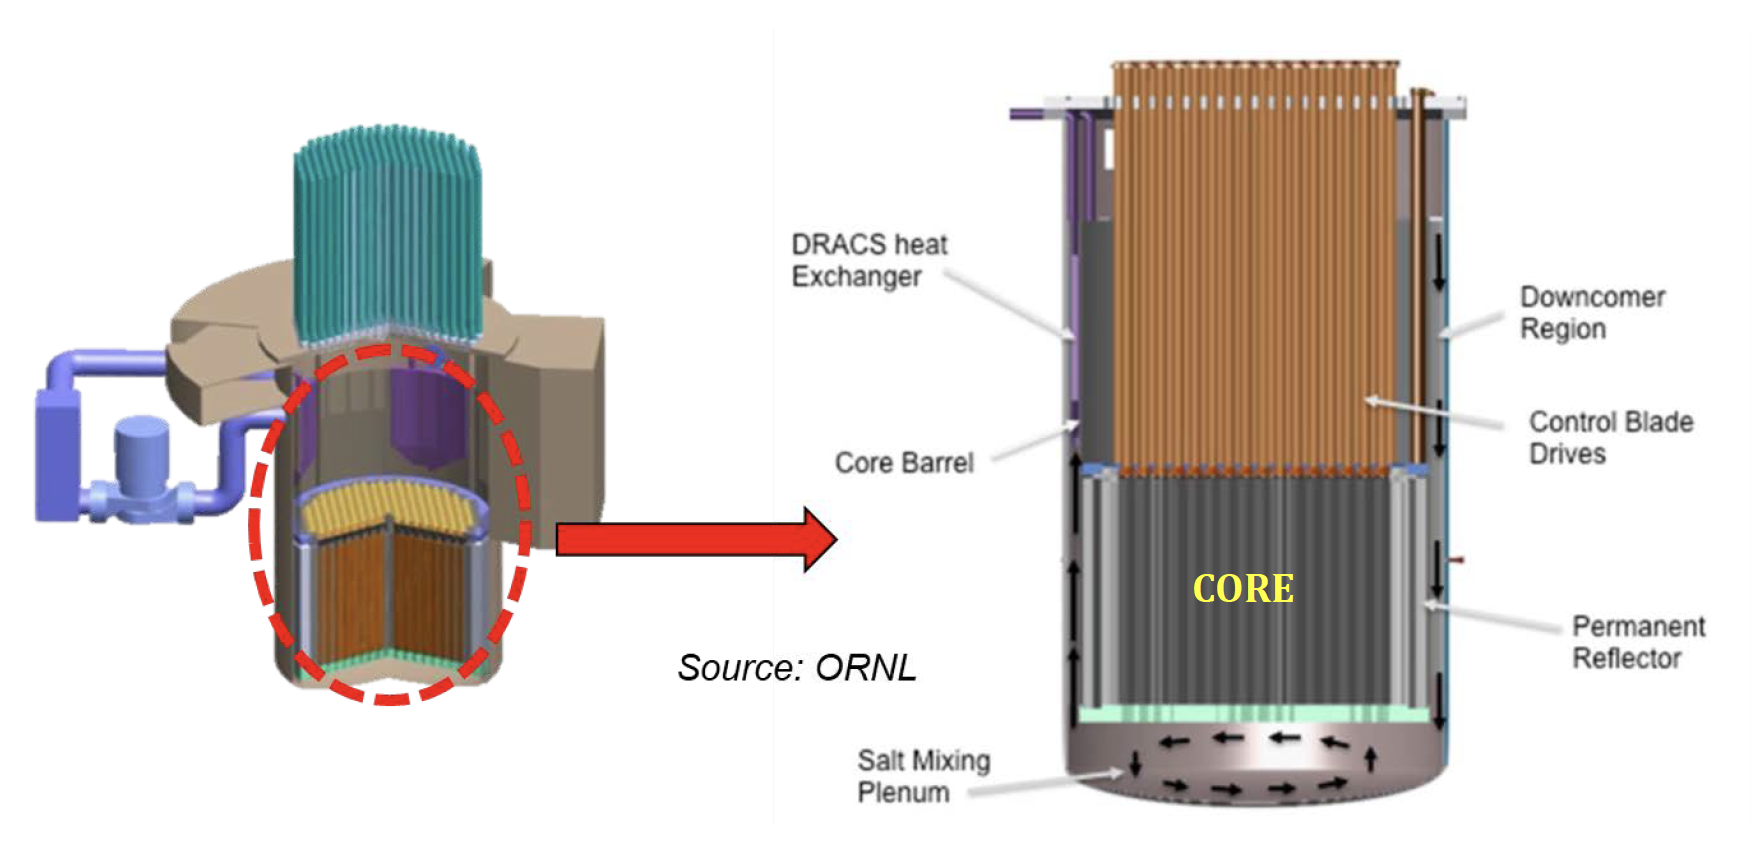
\includegraphics[width=0.5\linewidth]{../docs/figures/reactor-schematic.png} 
    \caption{\acrfull{AHTR} schematic (left) and vessel (right) reproduced from
    \cite{noauthor_fluoride_nodate}.}
\end{figure}
\end{frame}
\begin{frame}
  \frametitle{Advanced High Temperature Reactor Design}
    \begin{itemize}
      \item Design developed by Oak Ridge National Laboratory
      \item Prismatic FHR design with 252 hexagonal fuel assemblies consisting of 
      18 fuel planks arranged in 3 diamond-shaped sectors. 
    \end{itemize}
  \begin{figure}[]
    \centering
    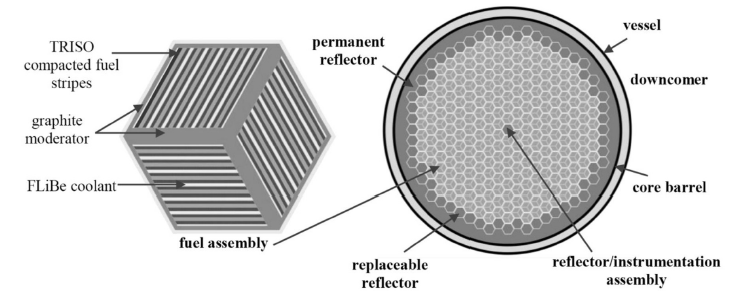
\includegraphics[width=0.9\linewidth]{../docs/figures/ahtr.png} 
    \caption{\acrlong{AHTR} fuel assembly (left) and core configuration (right) 
    reproduced from \cite{ramey_monte_2018}.}
    \label{fig:ahtr}
\end{figure}
\end{frame}

\begin{frame}
  \frametitle{Advanced High Temperature Reactor Geometry}
  The AHTR fuel has a \emph{triple heterogeneity}: hexagonal fuel elements with 
  fuel planks, and TRISO particles embedded in stripes within each plank.
  \begin{figure}[]
    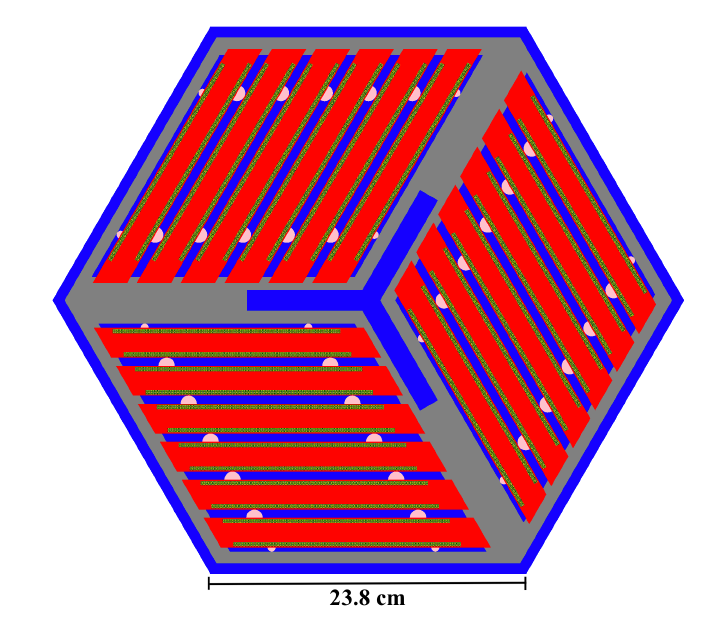
\includegraphics[width=0.5\linewidth]{figures/ahtr-assembly.png} 
    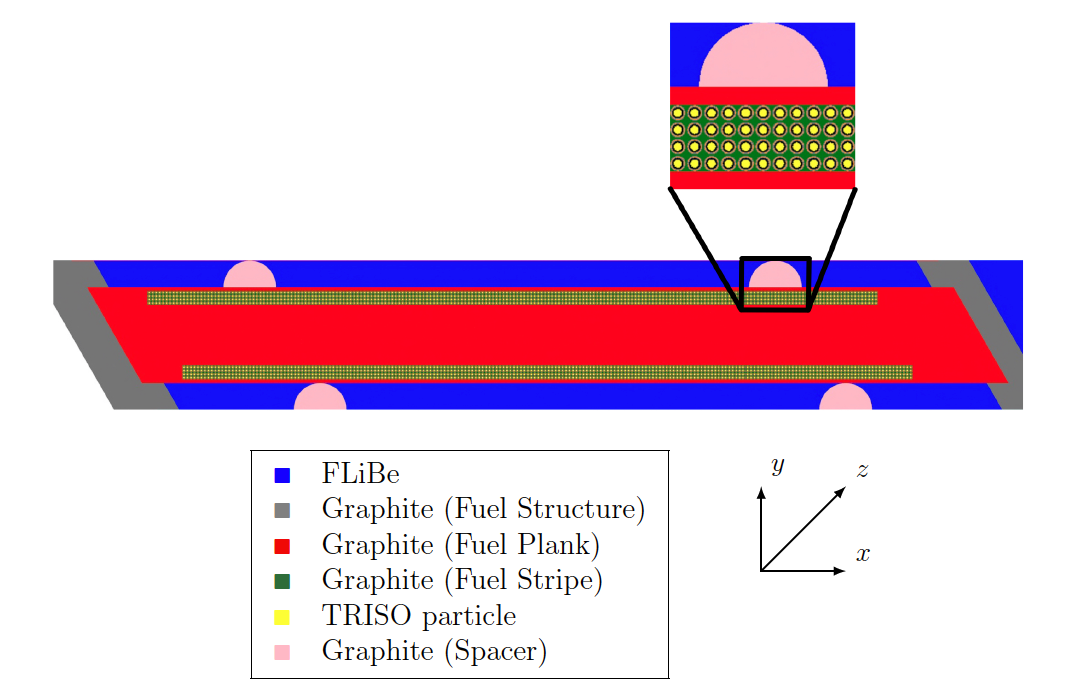
\includegraphics[width=0.5\linewidth]{figures/ahtr-plank.png} 
    \caption{AHTR fuel assembly with 18 fuel plates arranged in 
    three diamond-shaped sectors, with a central Y-shaped and external channel 
    graphite structure.}
\end{figure}
\end{frame}

\begin{frame}
  \frametitle{FHR Benchmark}
  \begin{itemize}
    \item The AHTR's fuel geometry's triple heterogeneity results in
    complex reactor physics and significant modeling challenges
    \item In 2019 the OECD-NEA initiated a FHR benchmark exercise. Its objective 
    is to identify the applicability, accuracy, and practicality of the latest 
    methods and codes to assess the current state of the art for FHR simulation 
    and modeling
  \end{itemize}
  \begin{figure}[]
    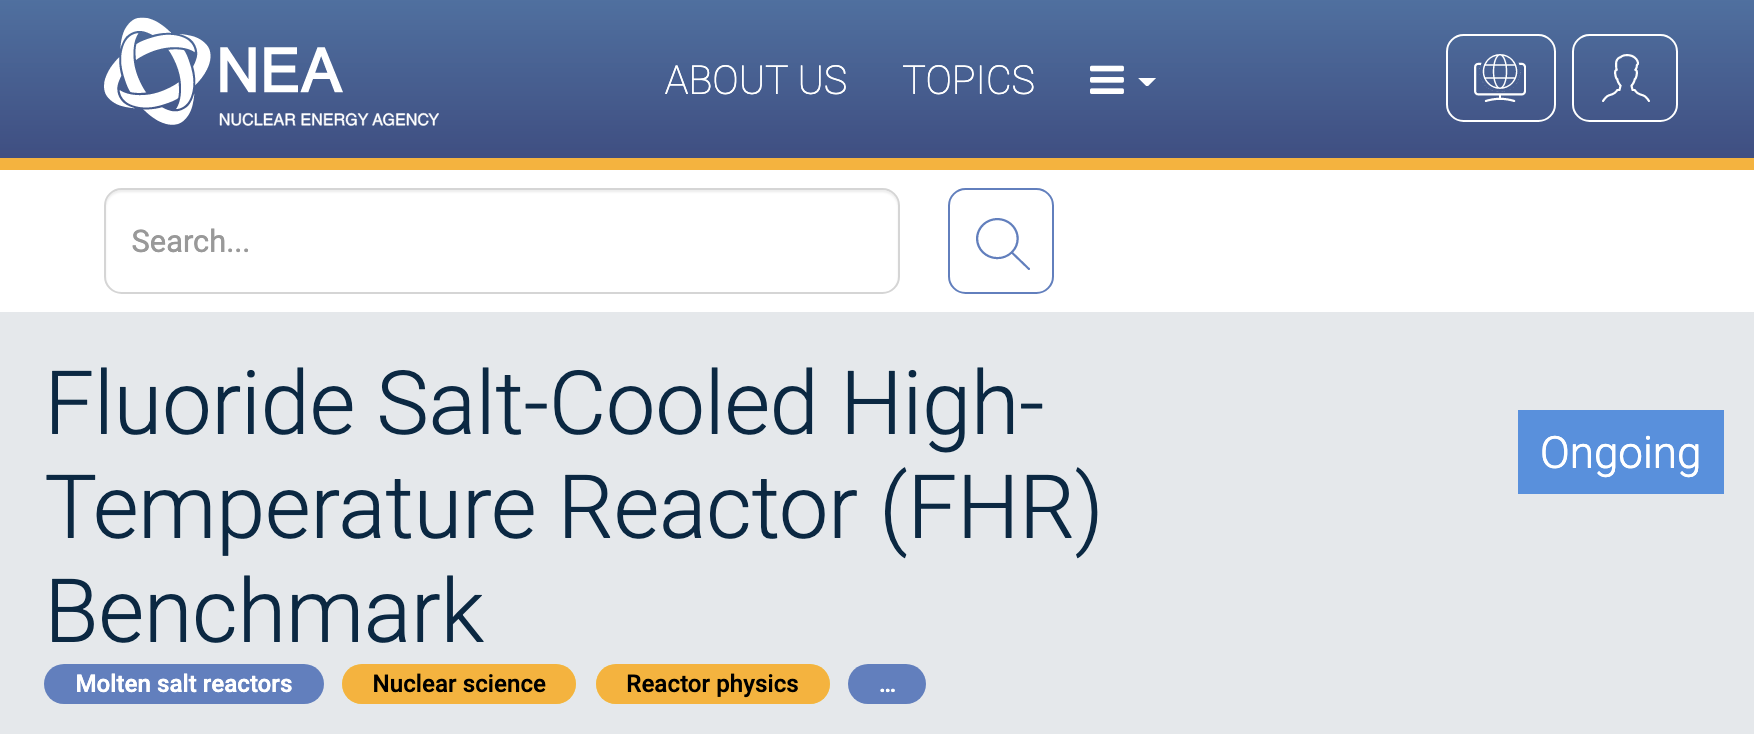
\includegraphics[width=0.7\linewidth]{figures/benchmark.png} 
    \caption{OECD NEA's FHR Benchmark \cite{petrovic_benchmark_2021}.}
\end{figure}
\end{frame}
